\section{Dated milestones with their assumptions exposed}
\label{sec:milestones}

The evidence supports measuring progress, not extrapolating a 50\% benchmark into a production
approval date. We separate four clocks: length capability, reliability qualification, evaluation, and
institutional change. Their parameters are explicit sensitivity inputs.

\subsection{Length capability: what three doublings would mean}

Use 8 May 2026 as a calendar anchor and choose $H_{80,0}=3$ human-hours for a planning calculation,
close to the 80\% horizon reported for the best model at that date \citep{metr2026a}. Extending the
historical seven-month doubling interval to the 80\% trajectory follows the similar trend reported by
\citet{kwa2025}; transferring it to gate work is a separate assumption. For target task length $D$,
\begin{equation}
T_{\mathrm{length}}(D)=d\,\bigl[\log_2(D/H_{80,0})\bigr]_{+}\ \text{months},\qquad d=7. \label{eq:length}
\end{equation}

\begin{table}[!htb]
\centering\small
\caption{Length milestones from a chosen three-hour 80\% anchor on 8 May 2026 and a seven-month
doubling interval. These are scenario dates, not observed gate capabilities or qualified deployment
dates.}
\label{tab:length}
\begin{tabular}{@{}r r r r l@{}}
\toprule
Target hours & Doublings & Exact months & Calendar months & Scenario date\\
\midrule
12 & 2.000 & 14.00 & 14 & 8 Jul 2027\\
24 & 3.000 & 21.00 & 21 & 8 Feb 2028\\
36 & 3.585 & 25.09 & 26 & 8 Jul 2028\\
\bottomrule
\end{tabular}
\end{table}

For twenty-four hours, three doublings give twenty-one months. That is a length milestone at the
selected 80\% criterion, not completion of a gate with a 20\% failure allowance. The formula
can be recalculated with an independently baselined gate horizon; changing the anchor changes the date
rather than the meaning of success. Figure~\ref{fig:doublings} shows how slower assumptions move the
milestone outward.

\begin{figure}[!htb]
\centering
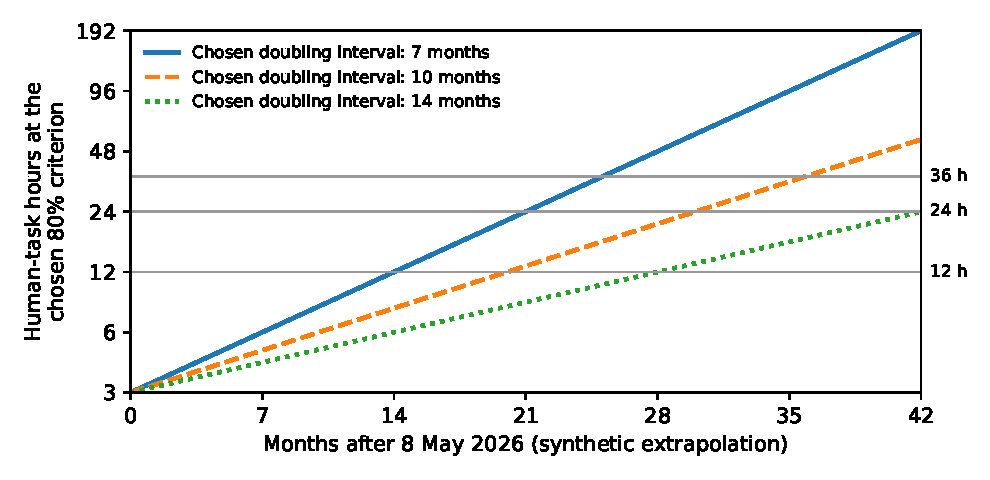
\includegraphics[width=0.84\linewidth]{figures/fig_doublings.pdf}
\caption{\textbf{How the assumed pace changes the length milestone.} All curves start from a chosen
three-hour horizon at 80\% success; none is a reconstructed METR series. A seven-month doubling reaches
twenty-four hours in twenty-one months. Reliability qualification and institutional delegation are
additional clocks.}
\label{fig:doublings}
\end{figure}

\subsection{The reliability tail has a separate clock and price}

Let $e_0=0.20$ be the scenario's initial error probability and $e^{*}$ a chosen qualification ceiling.
The number of tenfold error reductions required is
\begin{equation}
z=\log_{10}(e_0/e^{*}),\qquad T_{\mathrm{tail}}=\nu z,\qquad C_{\mathrm{tail}}/C_0=c^{z}. \label{eq:tail}
\end{equation}
Here $\nu$ is months per tenfold error reduction and $c$ its multiplicative resource-cost factor.
Neither is estimated from METR. Verification, retries, better evidence, or a better model could change
the costs differently; a nonzero irreducible error floor makes the target unreachable.

\begin{table}[!htb]
\centering\small
\caption{Reliability-tail sensitivity from initial error 0.20. Months per tenfold error reduction and
cost factors are independent, unestimated assumptions. The cost multiplier is relative to $C_0$, not a
quoted price.}
\label{tab:tail}
\begin{tabular}{@{}l r r r r r r r@{}}
\toprule
 & & \multicolumn{3}{c}{Tail months at $\nu=$} & \multicolumn{3}{c}{Cost multiplier at $c=$}\\
\cmidrule(lr){3-5}\cmidrule(l){6-8}
Error target & $z$ & 6 & 12 & 24 & 2 & 4 & 10\\
\midrule
$10^{-3}$ & 2.301 & 13.81 & 27.61 & 55.22 & 4.93 & 24.29 & 200.00\\
$5\times10^{-5}$ & 3.602 & 21.61 & 43.22 & 86.45 & 12.14 & 147.45 & 4,000.00\\
\bottomrule
\end{tabular}
\end{table}

The first row illustrates a 99.9\% gate criterion. A route budget of $10^{-3}$ over twenty possible
visits would instead require a conditional per-visit budget of $5\times10^{-5}$ in the simple
union-bound allocation; the second row shows how much more demanding that is. For a transparent serial
planning scenario,
\begin{equation}
T_{\mathrm{qualified}}=T_{\mathrm{length}}+T_{\mathrm{tail}}+T_{\mathrm{evaluation}}+T_{\mathrm{institution}}.
\label{eq:qualified}
\end{equation}
We use twelve months each for evaluation and institutional change only to illustrate their effect.
Tasks can progress in parallel in reality, while legal or information constraints can delay them
indefinitely.

\begin{table}[!htb]
\centering\small
\caption{Illustrative qualification calendar for a 24-hour task and a $10^{-3}$ error ceiling. Each
duration is rounded upward before calendar addition. Domain transfer, attainable error floors, and
legal permission remain separate requirements.}
\label{tab:calendar}
\begin{tabular}{@{}r r r r r l@{}}
\toprule
$\nu$ & Length & Tail & Evaluation + institution & Total months & Scenario date\\
\midrule
6 & 21 & 14 & 12 + 12 & 59 & 8 Apr 2031\\
12 & 21 & 28 & 12 + 12 & 73 & 8 Jun 2032\\
24 & 21 & 56 & 12 + 12 & 101 & 8 Oct 2034\\
\bottomrule
\end{tabular}
\end{table}

These scenarios make the content of the ten-year claim of Section~\ref{sec:testing} legible. The clocks
above start on 8 May 2026, whereas the cohort runs from 20 September 2026 to 20 September 2036 and its
twelve-month observation window must be completed inside that deadline. Qualified operation must
therefore begin by 20 September 2035, 112 months after the anchor. For a 24-hour work package,
$21+\nu z+24\le 112$ requires one tenfold error reduction every 29 months or faster at a $10^{-3}$
ceiling ($\nu\le 29.1$), and every 18 months or faster at $5\times10^{-5}$ ($\nu\le 18.6$). That pace
is the bet the law of gate substitution makes. A single 24-hour work package does not date a cohort: the deadline is
set by the slowest contract to qualify and by the dependencies the contracts share, including their
support.

\subsection{Route order is a hypothesis, not a relabelled trend}

We propose testing $W3\prec W1\prec W2$, Build before Buy before Integrate, as an adoption-order
hypothesis for comparable enterprises: builds can be designed to generate testable evidence; purchases
add supplier negotiation and evidence dependencies; integrations add inherited, inconsistently
documented state and lower repetition. An established SaaS procurement catalog could make Buy earlier than Build, and a highly
standardized acquisition program could reverse the final ordering. A calendar assessment should report,
for each gate, the observed horizon on its actual tasks, its error and labor components, qualification
status, and effective mandate. Updating a model name without those quantities is not evidence that a
milestone has been reached.
